 \begin{figure}[!t]
 \centering
 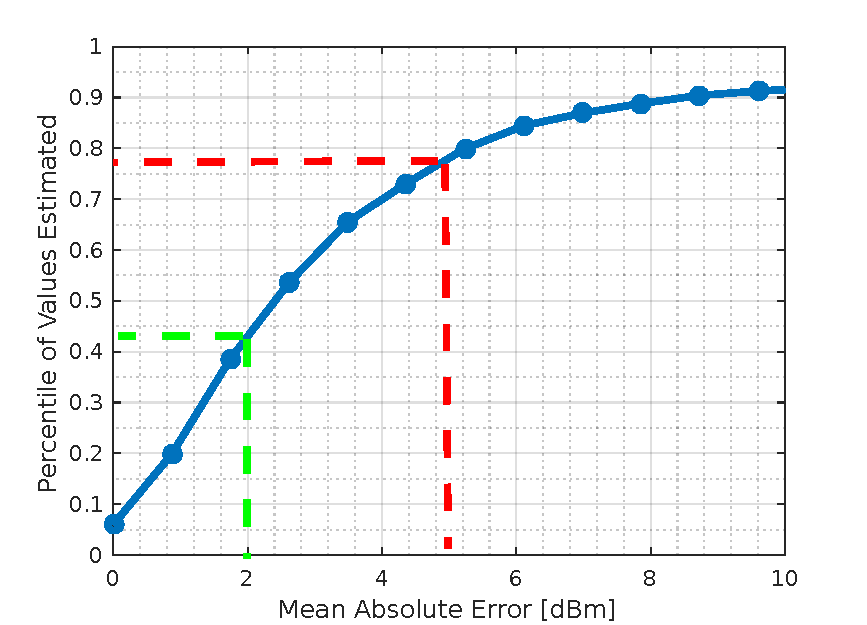
\includegraphics[width=\textwidth]{spectrum/mae_plot.pdf}
 \caption{Percentile of estimated wireless spectral power values against Mean Average Error of the estimates}
 \label{fig:mae_plot}
 \end{figure}
 
 \begin{figure*}[!t]
 \centering
 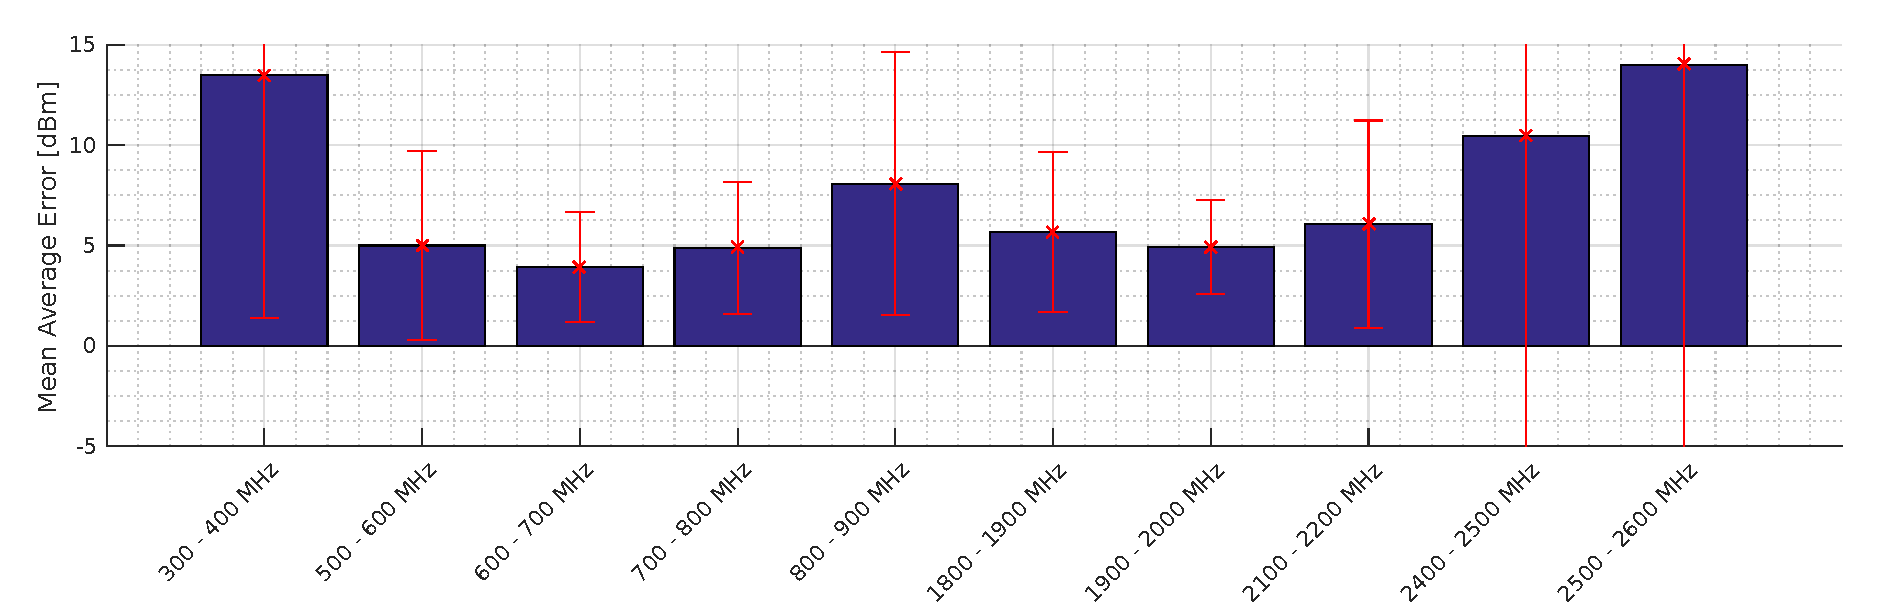
\includegraphics[width=\textwidth]{spectrum/freq_bin_plot.pdf}
 \caption{Mean Average Error of the estimated wireless spectral power for each 100 MHz frequency band}
 \label{fig:freq_bin_plot}
 \end{figure*}

 \begin{figure*}[!t]
 \centering
 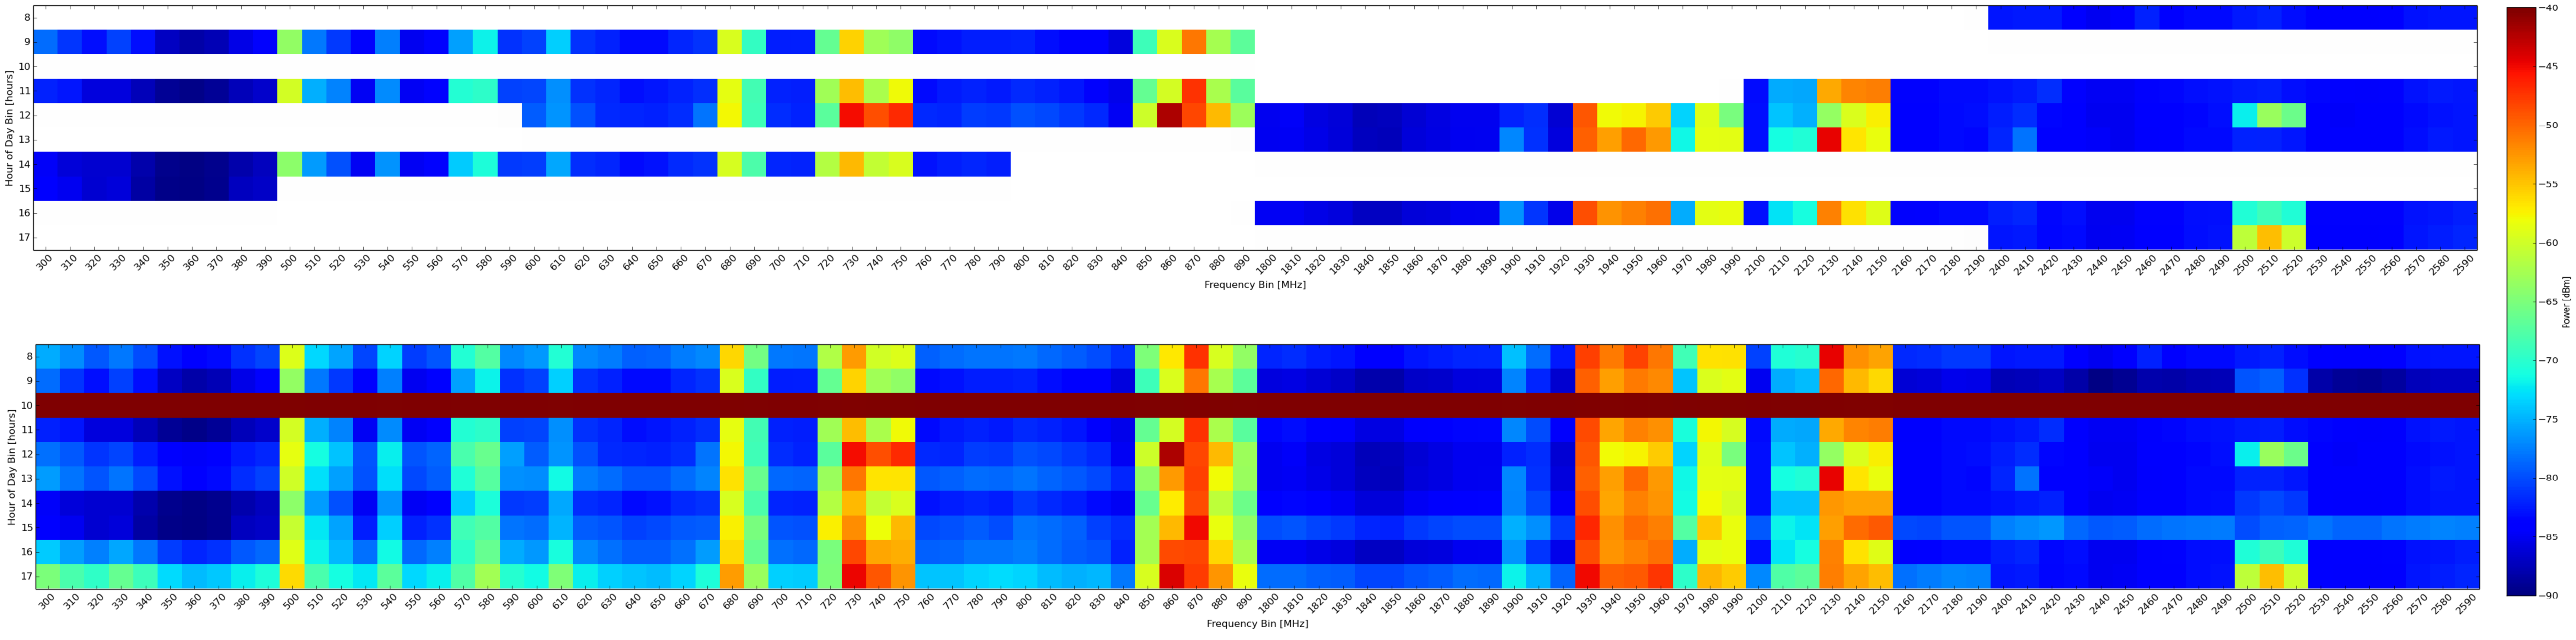
\includegraphics[width=\textwidth]{spectrum/comparison_image.pdf}
 \caption{Image Comparison of incomplete matrix (ground truth samples only) and uncovered matrix. X-Axis: Each entry along a row corresponds to the total power in a 10 MHz frequency band. Y-Axis: Each entry along a column corresponds to an hour of the day betwee 8 AM and 6 PM. Color: Each shade of color corresponds to a different power value as defined by the colorbar on the right}
 \label{fig:comparison_image}
 \end{figure*}

\section{Evaluation of Matrix Completion on Sparse Opportunistic Measurements}

Since the VScope data does not provide all entries in the matrix, I choose to evaluate this technique as follows:

\begin{itemize}
\item Construct the matrix for a single day, at a single location
\item Pick a 100 MHz frequnecy band for which measurement exists and hold-out the corresponding 10 samples
\item Run matrix completion on the rest of the samples and compare estimates with the 10 samples that were held out
\item Repeat this process for every 100 MHz frequency in the matrix and collect results about the estimation accuracy
\end{itemize}

I used this evaluation procedure for 5 different locations in Madison that observe both high and low foot traffic.
 For each location, I evaluate the algorithm for 4 different days (a total of 20 matrices and 20,000 entries).
 Since the chosen locations capture diversity in the underlying mobility models, I believe that this evaluation is representative of the general performance of this technique.


Figure \ref{fig:mae_plot} shows the percentile of data points against the mean absolute estimation error in dBm.
 This is useful to understand the prediction accuracy of the algorithm across frequency bands and builds confidence in the low-rank structure conjecture.
 The estimation error is < 2 dBm at the 40th percentile and < 5 dBm at the 80th percentile of the measurements.


Figure \ref{fig:freq_bin_plot} breaks up the error metrics by the frequency bins being studied.
 The mean absolute estimation error is < 5 dBm across most frequency bands.


Of course, these metrics are not fair if all measurements only indicate low spectral power (low occupancy) - if that was the case, then the problem is trivial and would not require such analyses.
 However, since I am considering cellular and Wi-Fi frequencies in a city setting low occupancy is almost never the case, depending on the exact band being examined.
 In Figure \ref{fig:comparison_image} I present a comparison between the measured sample matrix and the completed sample matrix using this method.
 Each column of the matrix corresponds to a 10 MHz frequency band and each row corresponds to an hour of the day from (8 AM - 6 PM).

We see that the power measurements show variation between -120 dBm to -50 dBm indicating that some bands do have meaningful activity.
 A glance at the "ground truth" measurements also indicates temporal variations hour-to-hour from which we are able to capture the hidden relationships to predict the missing samples.
 Additionally, we also witness one of the present drawbacks of this approach : when no samples are present in a one hour window, the algorithm is unable to "connect" the measurements for that hour with the known measurements and fails.
 This can be observed by the solid horizontal line for the hour between 10 AM and 11 AM.

